Algoritma Genetika (GA) merupakan salah satu metode heuristic yang merupakan cabang dari evolutionary algorithm, yaitu suatu teknik untuk memecahkan masalah-masalah optimasi yang rumit dengan menirukan proses evolusi mahluk hidup. GA terbukti sesuai digunakan untuk menyelesaikan masalah multi objektif. GA berkembang seiring dengan perkembangan teknologi informasi yang sangat pesat \cite{liu2016mining}, \cite{wei2015genetic}.

Algoritma ini banyak digunakan dalam bidang fisika, biologi, ekonomi, sosiologi dan lain-lain yang sering menghadapi masalah optimasi dengan model matematika yang kompleks atau bahkan sulit dibangun \cite{liu2016mining}.

\section{Implementasi Penjadwalan Algoritma Genetika di CodeIgniter}
\par Membuat CRUD dan beberapa table yang akan digunakan seperti pada tahap yang dilakukan sebelumnya, maka untuk mengimplementasikan algoritma genetika yaitu dengan cara melakukan konfigurasi pada model, controller dan views, langkah implementasi algoritma genetika yaitu sebagai berikut:
\begin{enumerate}
    \item Model Algoritma Genetika, pada folder model buat file baru denga nisi codingan seperti berikut, fungsinya adalah untuk memanggil semua table yang akan digunakan dalam algortima genetika. Pada codingan tersebut melakukan join terhadap beberapa table yang akan digunakan. Ingat pada saat melakukan join table pastikan table yang dibuat saling berelasi memiliki foreign key dan primary key pada masing-masing table.
		\begin{figure}[!htbp]
    		\centering
    		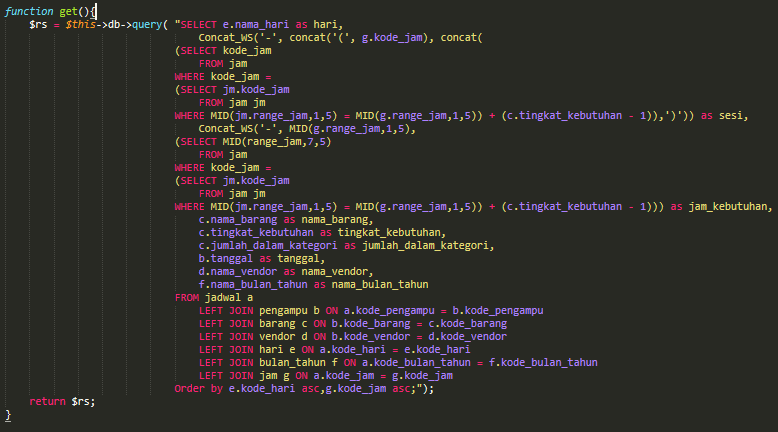
\includegraphics[width=0.7\textwidth]{figures/GA1.PNG}
    		\label{GA1}
		\end{figure}
		
	\item Selanjutnya adalah membuat codingan pada controller, buat file dengan nama genetik.php. pada file genetik.php tersebut didalamnya akan ada function seperti function ambildata, function inisialisasi, function cekfitness, function hitungfitness, function seleksi, function startcrossover, function mutase, dan function getindividu. Function tersebut dibuat secara berurut sesuai dengan urutan proses algoritma genetika.
	
	\item Untuk function ambildata dilakukan select data barang, tahun, bulan dan data vendor untuk dijadikan sebuah chromosome dalam bentuk variable
	
	\item Selanjutnya function inisialisasi, function ini dibuat untuk menentukan jam dan hari secara acak dengan menggunakan fungsi for dan if else
		\begin{figure}[!htbp]
    		\centering
    		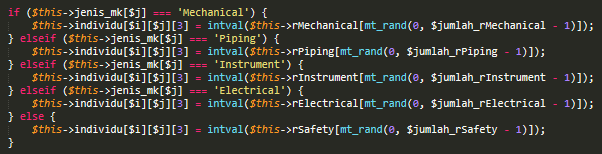
\includegraphics[width=0.7\textwidth]{figures/GA2.PNG}
    		\label{GA2}
		\end{figure}
	
	\item Function cekfitness, function ini dibuat untuk mencari jadwal yang bentrok sesuai dengan tingkat kebutuhan barang. Rumus yang digunakan dalam file ini adalah sebagai berikut:
	\par \verb|$fitness = floatval(1 / (1 + $penalty));|
	\par \verb|return $fitness;|
	\par Pada rumus tersebut mencari nilai penalty terhadap masing-masing individu, sehingga akan terbentuk nilai fitness terhadap setiap individu
	
	\item Setelah menemukan nilai fitness maka langkah selanjutnya adalah menghitung nilai fitness seperti pada gambar berikut
		\begin{figure}[!htbp]
    		\centering
    		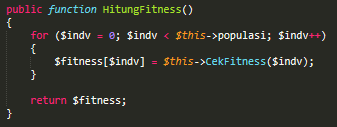
\includegraphics[width=0.5\textwidth]{figures/GA3.PNG}
    		\label{GA3}
		\end{figure}
		
	\item Selanjutnya adalah proses seleksi, untuk menari fitness terbaik dengan menggunakan proses rank selection pada pemrograman
		\begin{figure}[!htbp]
    		\centering
    		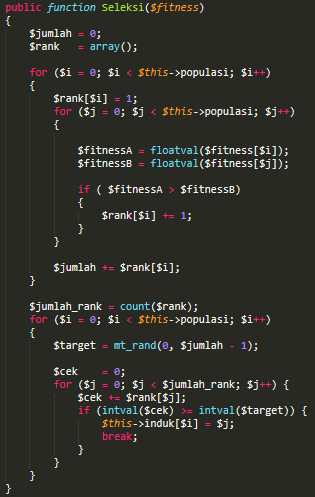
\includegraphics[width=0.5\textwidth]{figures/GA4.PNG}
    		\label{GA4}
		\end{figure}
		
	\item Kemudian langkah selanjutnya adalah melakukan crossover terhadap individu yang tidak terpilih guna untuk mencari populasi baru
		\begin{figure}[!htbp]
    		\centering
    		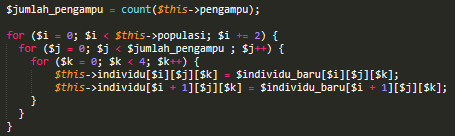
\includegraphics[width=0.5\textwidth]{figures/GA5.PNG}
    		\label{GA5}
		\end{figure}
		
	\item Function mutasi, pada function ini ketika nilai random kurang dari nilai probalitas Mutasi, maka terjadi penggantian komponen
		\begin{figure}[!htbp]
    		\centering
    		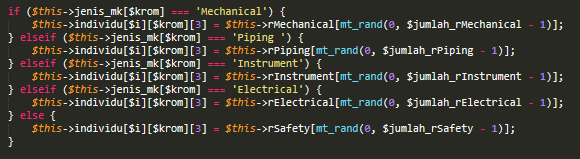
\includegraphics[width=0.8\textwidth]{figures/GA6.PNG}
    		\label{GA6}
		\end{figure}
		
	\item Function terakhir adalah function getindividu. Function ini berguna untuk mengambil hasil akhir atau memberikan solusi terbaik dari setiap proses awal sampai akhir
		\begin{figure}[!htbp]
    		\centering
    		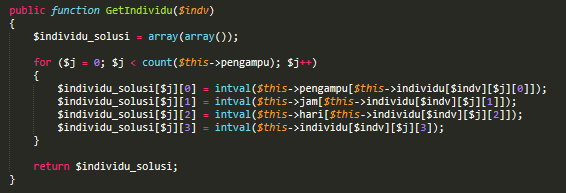
\includegraphics[width=0.7\textwidth]{figures/GA7.PNG}
    		\label{GA7}
		\end{figure}
		
	\item Setelah file genetika.php selesai, simpan file tersebut kemudian buat file controller dalam folder yang sama yang kemudian akan include dengan file genetic.php atau file algoritma genetika

    \item Kemudian includkan genetic.php pada file ini
		\begin{figure}[!htbp]
    		\centering
    		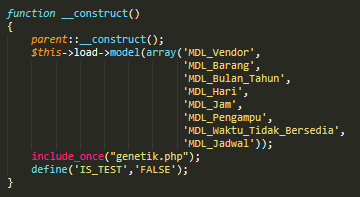
\includegraphics[width=0.7\textwidth]{figures/GA8.PNG}
    		\label{GA8}
		\end{figure}
	
	\item Buat function \verb|index_jadwal| untuk melakukan proses view jadwal pada aplikasi web, berikut isi dari function \verb|index_jadwal|
        \begin{enumerate}
            \item Panggil semua data yang akan digunakan untuk proses algoritma genetika proses
        		\begin{figure}[!htbp]
            		\centering
            		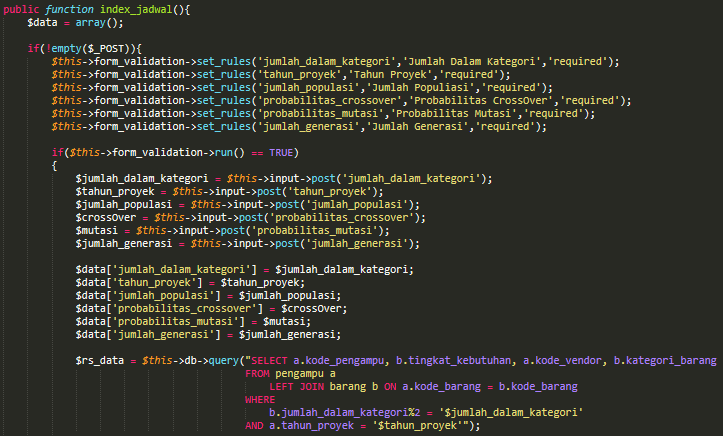
\includegraphics[width=0.5\textwidth]{figures/GA9.PNG}
            		\label{GA9}
        		\end{figure}
        	
        	\item Kelola data dalam bentuk variable untuk mencari hasil terbaik
        		\begin{figure}[!htbp]
            		\centering
            		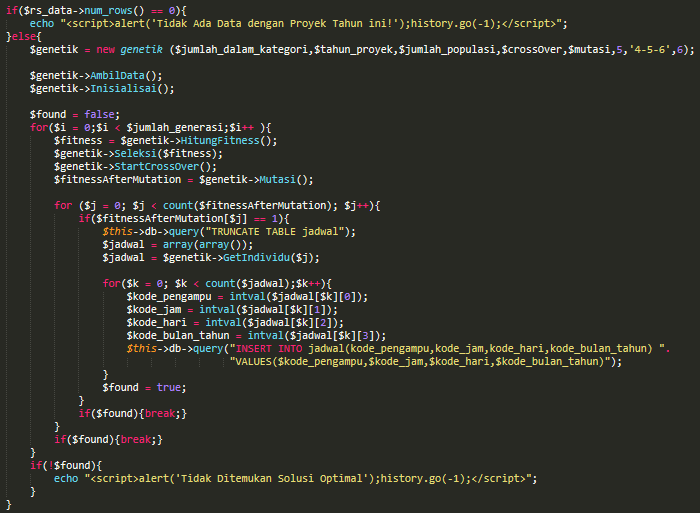
\includegraphics[width=0.6\textwidth]{figures/GA10.PNG}
            		\label{GA10}
        		\end{figure}
        		
        	\item Setelah data di proses, tampilkan data dalam bentuk web, dan hasil di input langsung kedalam database
        		\begin{figure}[!htbp]
            		\centering
            		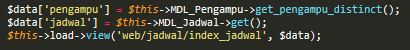
\includegraphics[width=0.6\textwidth]{figures/GA11.PNG}
            		\label{GA11}
        		\end{figure}
        \end{enumerate}
        		
    	\item Selanjutnya buat file baru pada folder application/views/\verb|index_jadwal| dan buat desain untuk tampilan hasil penjadwalan nanti. Dan buat beberapa button atau fungsi untuk dilemparkan ke function controller yang sudah dibuat tadi.
    		\begin{figure}[!htbp]
        		\centering
        		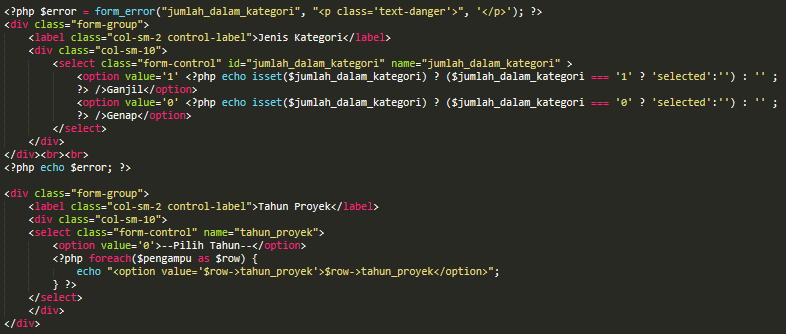
\includegraphics[width=0.6\textwidth]{figures/GA12.PNG}
        		\label{GA12}
    		\end{figure}
    		\begin{figure}[!htbp]
        		\centering
        		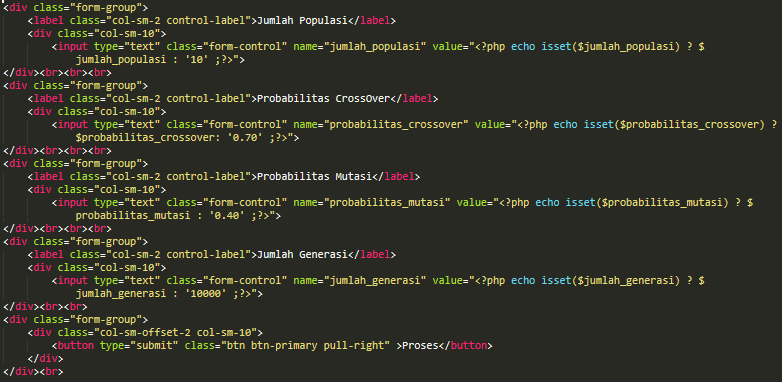
\includegraphics[width=0.6\textwidth]{figures/GA13.PNG}
        		\label{GA13}
    		\end{figure}
    		
    	\item Kemudian tambahkan tampilan table untuk hasil jadwal eksekusi penjadwalan nanti
    		\begin{figure}[!htbp]
        		\centering
        		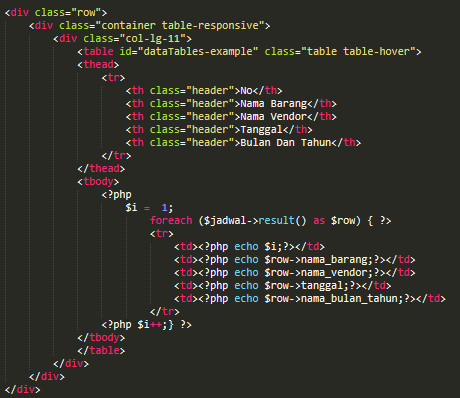
\includegraphics[width=0.5\textwidth]{figures/GA14.PNG}
        		\label{GA14}
    		\end{figure}
    	
    	\item Setelah semua selesai, simpan file tersebut kemudian jalankan aplikasi
    	
        \item Berikut hasil dari aplikasi penjadwalan algoritma genetika
    		\begin{figure}[!htbp]
        		\centering
        		\caption{Hasil Penjadwalan Algoritma Genetika}
        		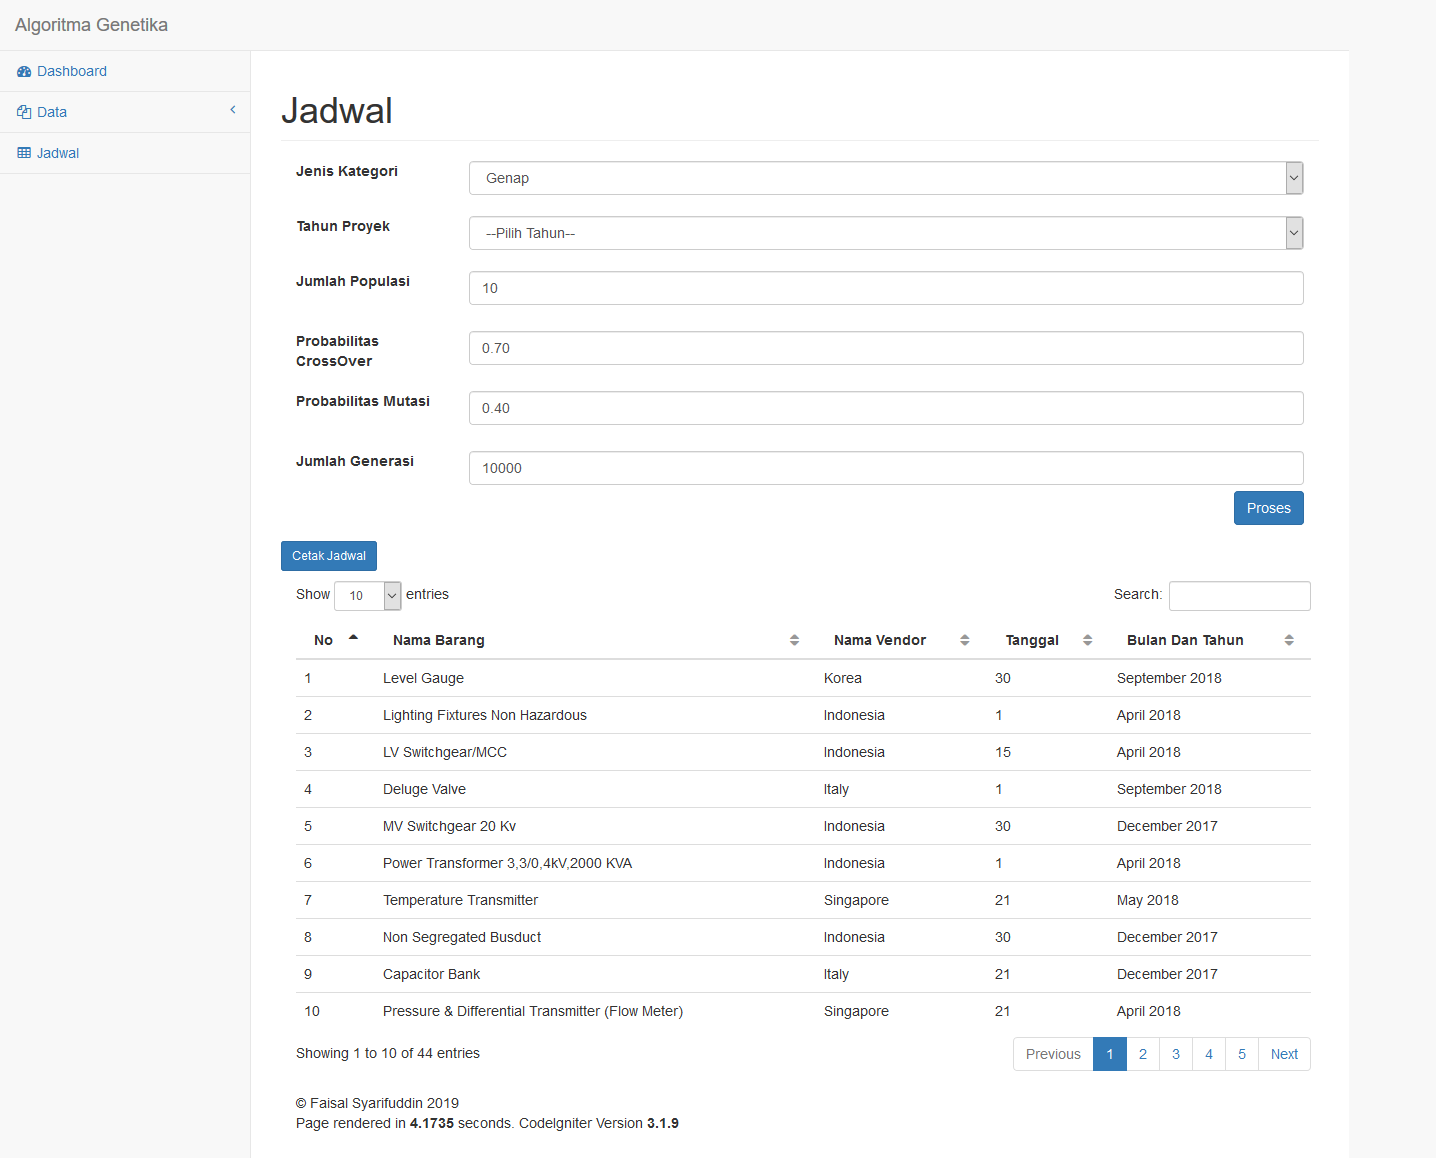
\includegraphics[width=0.6\textwidth]{figures/GA15.png}
        		\label{GA15}
    		\end{figure}
\end{enumerate}